\documentclass{beamer}

\usetheme[progressbar=frametitle]{metropolis}
\usepackage{appendixnumberbeamer}
\usepackage{booktabs}
\usepackage{amsmath}
\usepackage{amssymb}
\usepackage{tcolorbox}
\usepackage{tikz}
\usetikzlibrary{bayesnet}
\definecolor{metropolisblue}{RGB}{39, 59, 94}



% Begin document
\begin{document}


% Title page
\title{Maximum Likelihood Estimation for Linear and Logistic Regression}
\author{Nipun Batra}
\date{\today}
\institute{IIT Gandhinagar}
\maketitle
\setbeamercovered{invisible}
\begin{frame}
    \frametitle{Agenda}
    \tableofcontents[hidesubsections]
    \end{frame}
    




\section{MLE for Linear Regression}
\begin{frame}{MLE for Linear Regression}
\begin{figure}
                \centerline{\includegraphics[scale=0.8]{../figures/mle/true_function_lin_reg.pdf}}
\end{figure}
\end{frame}
\begin{frame}{MLE for Linear Regression}
\begin{figure}
                \centerline{\includegraphics[scale=0.8]{../figures/mle/true_function_noise_lin_reg.pdf}}
\end{figure}
\end{frame}
\begin{frame}{MLE for Linear Regression}
\begin{figure}
                \centerline{\includegraphics[scale=0.8]{../figures/mle/true_function_noise_normal_lin_reg.pdf}}
\end{figure}
\end{frame}
\begin{frame}
Let us assume we have a dataset $D = \{(x_1, y_1), (x_2,y_2), \ldots, (x_n, y_n)\}$, where $x_i\in R^d, y_i\in R$. 

\vspace{10pt}
\pause We consider a regression problem with the likelihood function: $p(y|x) = \mathbb{N}(y|f(x), \sigma^2)$.\\
\end{frame}

\begin{frame}
The functional relationship between $x$ and $y$ is given as $y = f(\bold{x})+\epsilon$ where $\epsilon\sim \mathbb{N}(0, \sigma^2).$ \\ 

\vspace{10pt}
\pause where $f(\bold{x}) = x^T\theta$ for linear regression\\ 

\vspace{10pt}
\pause 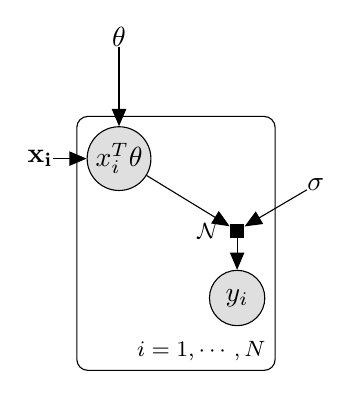
\begin{tikzpicture}
                
                
    \node[obs]                               (xit) {$x_i^T\theta$};
    \node[obs, below=1 of xit, xshift = 1.5cm] (yi) {$y_i$};
    \node[const, xshift=-1cm](xi) {$\mathbf{x_i}$};
    \node[const, above=1 of xit](theta)
    {$\mathbf{\theta}$};
    
    \factor[above=of yi] {y-f} {left:${\mathcal{N}}$} {} {} ; %
            \node[const, above=1 of yi, xshift=1cm] (sigma) {$\mathbf{\sigma}$};
    \plate{}{(xit)(yi)}{$i = 1, \cdots, N$};
    \edge{theta}{xit}
    \edge{xit}{y-f}
    \edge{sigma}{y-f}
    \edge{xi}{xit}
    \edge{y-f}{yi}
            
            
\end{tikzpicture}

\end{frame}


\begin{frame}{Likelihood for linear regression}
    Likelihood is generally given as: 
    \begin{equation}
        P(D|\theta) 
    \end{equation}
    \vspace{10pt}
    \pause Our data is: $D = \{(x_1, y_1), (x_2,y_2), \ldots, (x_n, y_n)\}$
    \vspace{10pt}

    \pause Note: For purposes of computing likelihood, we assume that the input (x) is fixed and variation is only in the output (y).

    \vspace{10pt}
    \pause Our likelihood function (Normal distribution) is given by:
    \begin{equation}
    P(\mathcal{Y}|\mathcal{X},\theta) = p(y_1,\ldots,y_n|x_1,\ldots,x_n,\theta) = \prod_{i=1}^n p(y_i|x_i, \theta) 
    \end{equation}
\end{frame}
    
\begin{frame}{Likelihood for linear regression}
    The MLE equation is given by:
    \begin{equation}
        \theta_{MLE}\in \arg_{\theta} \max p(Y|X,\theta)
    \end{equation}
    \pause Maximizing the likelihood $\equiv$ Maximizing the log likelihood $\equiv$ Minimizing the negative log likelihood.\\
    \pause Taking the negative log, we get:
    \vspace{10pt}
    \pause \begin{align*}
        -\log p(\mathcal{Y} \mid \mathcal{X}, \boldsymbol{\theta}) &= -\log \prod_{i=1}^N p(y_i \mid \boldsymbol{x}_i, \boldsymbol{\theta}) \\
        &= -\sum_{i=1}^N \log p(y_i \mid \boldsymbol{x}_i, \boldsymbol{\theta})
    \end{align*}
    \pause For a given point $(x_i, y_i),$
    \pause \begin{align*}
        -\log p(y_i \mid \boldsymbol{x}_i, \boldsymbol{\theta}) = \frac{1}{2 \sigma^2} \left(y_i - \boldsymbol{x}_i^{\top} \boldsymbol{\theta}\right)^2 + \text{const}
    \end{align*}
    \end{frame}
    

\begin{frame}{Likelihood for linear regression}
Thus the negative log likelihood is simplified to:
\begin{align*} \mathcal{NLL}(\boldsymbol{\theta}) & :=\frac{1}{2 \sigma^2} \sum_{i=1}^N\left(y_i-\boldsymbol{x}_i^{\top} \boldsymbol{\theta}\right)^2 \\ & =\frac{1}{2 \sigma^2}(\boldsymbol{y}-\boldsymbol{X} \boldsymbol{\theta})^{\top}(\boldsymbol{y}-\boldsymbol{X} \boldsymbol{\theta})=\frac{1}{2 \sigma^2}\|\boldsymbol{y}-\boldsymbol{X} \boldsymbol{\theta}\|^2\end{align*}\\
\pause \begin{tcolorbox}[colback=metropolisblue!5,colframe=metropolisblue,title=Negative Log Likelihood for Linear Regression]     
        NLL is proportional to:
        \begin{equation*}
            \frac{1}{2 \sigma^2}\|\boldsymbol{y}-\boldsymbol{X} \boldsymbol{\theta}\|^2
        \end{equation*}
    \end{tcolorbox}
\pause This is the same as the squared error loss. 
\end{frame}


\begin{frame}
    To minimize $NLL(\theta)$, we differentiate with respect to $\theta$. 
   \pause  \begin{equation}
        \theta = (X^TX)^{-1}X^Ty
    \end{equation}
    \pause \begin{tcolorbox}[colback=metropolisblue!5,colframe=metropolisblue,title=Maximum Likelihood Estimate for $\theta$]
        MLE of $\theta$, denoted as $\hat{\theta}_{\text{MLE}}$, is given by:
        \begin{equation*}
            \hat{\theta}_{\text{MLE}} = (X^TX)^{-1}X^Ty
        \end{equation*}
    \end{tcolorbox}
\end{frame}

\begin{frame}{MLE for $\sigma^2$}
    Self Study, Reference: MML book
    $$
\sigma_{\mathrm{ML}}^2=\frac{s}{N}=\frac{1}{N} \sum_{n=1}^N\left(y_n-\boldsymbol{\phi}^{\top}\left(\boldsymbol{x}_n\right) \boldsymbol{\theta}\right)^2
$$
Therefore, the maximum likelihood estimate of the noise variance is the empirical mean of the squared distances between the noise-free function values $\phi^{\top}\left(\boldsymbol{x}_n\right) \boldsymbol{\theta}$ and the corresponding noisy observations $y_n$ at input locations $\boldsymbol{x}_n$.
    
\end{frame}


\begin{frame}
    \begin{figure}
                \centerline{\includegraphics[scale=0.8]{../figures/mle/lin_reg_slider_1.pdf}}
\end{figure}
\end{frame}
\begin{frame}
    \begin{figure}
                \centerline{\includegraphics[scale=0.8]{../figures/mle/lin_reg_slider_2.pdf}}
\end{figure}
\end{frame}
\begin{frame}
    \begin{figure}
                \centerline{\includegraphics[scale=0.8]{../figures/mle/lin_reg_slider_3.pdf}}
\end{figure}
\end{frame}
\section{MLE for Logistic Regression}


\begin{frame}{Logistic Regression and Coin Toss}

    Coin Toss: We are given coin tosses: $D = \{y_1, y_2, \ldots, y_n\}$, where $y_i\in \{0,1\}$. \\
    \vspace{10pt}
    \pause  Logistic regression: We are given a dataset: $D = \{(x_1, y_1), (x_2,y_2), \ldots, (x_n, y_n)\}$, where $x_i\in R^d, y_i\in \{0,1\}$. \\

    

    

    
\end{frame}

\begin{frame}{Logistic Regression and Coin Toss}

    Coin Toss: The probability of getting a head (class 1) is given by $\theta$, i.e.
    $$p(y=1) = \theta$$
    \vspace{10pt}
    \pause 
    Logistic regression: The probability that a given input $x$ belongs to class 1 is given by:
    $$p(y=1|x) = \sigma(x^T\theta)$$
\end{frame}

\begin{frame}{Logistic Regression and Coin Toss}

    Coin Toss: We can say 
    $$y \sim \text{Bernoulli}(\theta)$$
    \vspace{10pt}
    \pause 
    Logistic regression: We can say
    $$y \sim \text{Bernoulli}(\sigma(x^T\theta))$$
\end{frame}\

\begin{frame}{Logistic Regression and Coin Toss: Graphical model}

    Coin Toss
    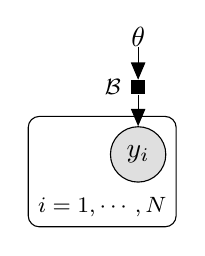
\begin{tikzpicture}
                
                
        \node[obs]                               (xn) {$y_i$};
        \factor[above=of xn] {y-f} {left:${\mathcal{B}}$} {} {} ; %
        \node[const, above=1 of xn] (theta) {$\mathbf{\theta}$};
        \plate{}{(xn)}{$i = 1, \cdots, N$};
        
        
        
        \edge {y-f} {xn} ; %
        \edge {theta} {y-f} ; %
        
        
    \end{tikzpicture}
    
    \pause Logistic Regression

    \begin{tikzpicture}

        \node[obs] (x_i_theta) {$x_i^T\theta$};
        \node[const, left=of x_i_theta] (xi) {$\mathbf{x_i}$};
        \node[const, above=of x_i_theta] (theta) {$\mathbf{\theta}$};
        \node[const, right=of x_i_theta] (pxi) {$p(x_i)$};
        \factor[const, right=of pxi] (beta) {$\mathcal{B}$};
        \node[obs, right=of beta] (yi_out) {$y_i$};
        \plate {plate1} {(xi)(x_i_theta)(yi_out)} {$i = 1, \cdots, N$};
        
        \edge {xi} {x_i_theta};
        \draw[->] (theta) -- (x_i_theta);
        \draw[->] (x_i_theta) -- node[above] {$\sigma$} (pxi); % Adding "sigma" text
        \draw[->] (pxi) -- (beta);
        \draw[->] (beta) -- (yi_out);
        
        \end{tikzpicture}
        
\end{frame}
    



\begin{frame}{Logistic Regression and Coin Toss}

    Coin Toss: Likelihood is given by:
    $$L(\theta) = \prod_{i=1}^n \theta^{y_i}(1-\theta)^{1-y_i}$$
    \vspace{10pt}
    \pause 
    Logistic regression: Likewise, likelihood is given by:
    $$L(\theta) = \prod_{i=1}^n \sigma(x_i^T\theta)^{y_i}(1-\sigma(x_i^T\theta))^{1-y_i}$$
\end{frame}

\begin{frame}{Logistic Regression and Coin Toss}

    Coin Toss: Likelihood is given by:
    $$L(\theta) = \prod_{i=1}^n \theta^{y_i}(1-\theta)^{1-y_i}$$
    \vspace{10pt}
    \pause 
    Logistic regression: Likewise, likelihood is given by:
    \pause To simplify, we can write: $\hat{y_i} = \sigma(x_i^T\theta)$
    \pause Thus, likelihood is given by:
    $$L(\theta) = \prod_{i=1}^n \hat{y_i}^{y_i}(1-\hat{y_i})^{1-y_i}$$
\end{frame}

\begin{frame}{Logistic Regression and Coin Toss}

    Coin Toss: Log likelihood is given by:
    $$\log(L(\theta)) = \sum_{i=1}^n y_i\log(\theta) + (1-y_i)\log(1-\theta)$$
    \vspace{10pt}
    \pause 
    Logistic regression: Likewise, log likelihood is given by:
    $$\log(L(\theta)) = \sum_{i=1}^n y_i\log(\hat{y_i}) + (1-y_i)\log(1-\hat{y_i})$$
\end{frame}

\begin{frame}{Negative Log Likelihood for Logistic Regression}
    \begin{tcolorbox}[colback=metropolisblue!5,colframe=metropolisblue,title=Negative Log Likelihood for Logistic Regression]
        NLL is proportional to:
        \begin{equation*}
            -\sum_{i=1}^n y_i\log(\hat{y_i}) + (1-y_i)\log(1-\hat{y_i})
        \end{equation*}
        which is the same as the binary cross entropy loss function.
    \end{tcolorbox}
    
\end{frame}

\begin{frame}{Extending binary classification to $K$-class classification}
    For binary classification, we have a sigmoid function.\\
    $p(y=1|x) = \sigma(x^T\theta)$\\
    \vspace{10pt}
    \pause For multi-class classification, we have a softmax function.\\
    $p(y=i|x) = \frac{e^{x^T\theta_i}}{\sum_{j=1}^Ke^{x^T\theta_j}}$\\

    
    
\end{frame}

\begin{frame}{Extending binary classification to multi-class classification}
   Self-Study: Derive the negative log likelihood for multi-class classification and show that it is the same as the cross entropy loss function.

    
\end{frame}

\begin{frame}{MLE for Logistic Regression}
% \begin{tikzpicture}
                
                
%     \node[obs]                               (y_i) {$x_i\theta$};
%     \node[const, xshift=-1cm](xi) {$\mathbf{x_i}$};
%     \node[const, above=1 of yi](theta){$\mathbf{\theta}$};
%     \node[const, xshift=1.5cm](pxi) {$p(x_i)$}
%     \node[const, xshift=2.5cm](beta) {$\beta$}
%     \plate{}{(yi)}{$i = 1, \cdots, N$};
%     \edge{yi}{pxi}
%     \edge{pxi}{beta}
%     \edge{theta}{yi}
%     \edge{xi}{yi}
            
            
% \end{tikzpicture}\\

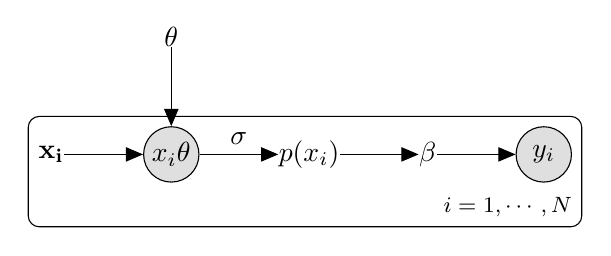
\begin{tikzpicture}

\node[obs] (x_i_theta) {$x_i\theta$};
\node[const, left=of x_i_theta] (xi) {$\mathbf{x_i}$};
\node[const, above=of x_i_theta] (theta) {$\mathbf{\theta}$};
\node[const, right=of x_i_theta] (pxi) {$p(x_i)$};
\node[const, right=of pxi] (beta) {$\beta$};
\node[obs, right=of beta] (yi_out) {$y_i$};
\plate {plate1} {(xi)(x_i_theta)(yi_out)} {$i = 1, \cdots, N$};

\draw[->] (xi) -- (x_i_theta);
\draw[->] (theta) -- (x_i_theta);
\draw[->] (x_i_theta) -- node[above] {$\sigma$} (pxi); % Adding "sigma" text
\draw[->] (pxi) -- (beta);
\draw[->] (beta) -- (yi_out);

\end{tikzpicture}





Binary Classification:\\
The probability distribution in case of Logistic Regression considering two classes is Bernoulli distribution but there is a slight difference. The probability is now the output of the logistic function.
Parameters are $\theta=[\theta_0,\theta_1]$.
\begin{equation}
p = P(Y=1|X) = \frac{1}{1+e^{-(\theta_0+\theta_1X)}}
\end{equation}


\end{frame}

\begin{frame}
Rewriting the likelihood in this manner:
\begin{align*}
    L(\theta)&= \prod_{y_i=1}p(x_i)\prod_{y_i=0}(1-p(x_i))\\
    &=\prod\left(p(x_i)^{y_i}(1-p(x_i))^{1-y_i}\right)
\end{align*}
Taking log on both sides:\\
\begin{align*}
    \log(L(\theta)) &= \sum_{i=1}^n y_i\log(p(x_i)) + (1-y_i)\log(1-p(x_i))
\end{align*}
If we multiply this by $-\frac{1}{n},$this is nothing but the binary cross entropy loss function!
\end{frame}
\begin{frame}
    \begin{figure}
                \centerline{\includegraphics[scale=0.8]{../figures/mle/log_reg_slider_1.pdf}}
\end{figure}
\end{frame}
\begin{frame}
    \begin{figure}
                \centerline{\includegraphics[scale=0.8]{../figures/mle/log_reg_slider_2.pdf}}
\end{figure}
\end{frame}
\begin{frame}
    \begin{figure}
                \centerline{\includegraphics[scale=0.8]{../figures/mle/log_reg_slider_3.pdf}}
\end{figure}
\end{frame}

\begin{frame}{Coin toss V/s Binary Logistic Regression}
\begin{center}
    \begin{tabular}{|c|c|}
    \hline
    \textbf{Coin toss} & \textbf{Binary Logistic Regression} \\
    \hline
    Likelihood=$\theta^{t}(1-\theta)^{1-t}$& Likelihood=$(\sigma(x^T\theta))^t(1-\sigma(x^T\theta))^{1-t}$ \\
    \pause
    Outcome is Head/Tail & Outcome is out of two possible classes \\
    \pause
    Parameter is scalar & Parameter is vector with two values\\
    \hline
  \end{tabular}
\end{center}    
\end{frame}

\begin{frame}


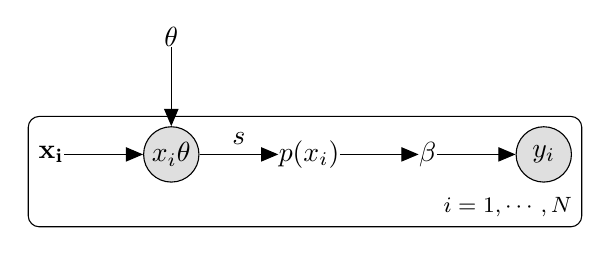
\begin{tikzpicture}

\node[obs] (x_i_theta) {$x_i\theta$};
\node[const, left=of x_i_theta] (xi) {$\mathbf{x_i}$};
\node[const, above=of x_i_theta] (theta) {$\mathbf{\theta}$};
\node[const, right=of x_i_theta] (pxi) {$p(x_i)$};
\node[const, right=of pxi] (beta) {$\beta$};
\node[obs, right=of beta] (yi_out) {$y_i$};
\plate {plate1} {(xi)(x_i_theta)(yi_out)} {$i = 1, \cdots, N$};

\draw[->] (xi) -- (x_i_theta);
\draw[->] (theta) -- (x_i_theta);
\draw[->] (x_i_theta) -- node[above] {$s$} (pxi); % Adding "sigma" text
\draw[->] (pxi) -- (beta);
\draw[->] (beta) -- (yi_out);

\end{tikzpicture}





Multi-class Classification:\\
The probability distribution in case of Logistic Regression considering more than two classes is Categorical distribution. The probability is now the output of the softmax function.
Parameters are $\theta=[\theta_0,\theta_1,\ldots, \theta_k]$.
\begin{equation}
p = P(Y=i|X) = \frac{e^{\theta x_i}}{\sum_{j=1}^ne^{\theta x_j}}
\end{equation}


\end{frame}
\begin{frame}
Now:
\begin{align*}
    L(\theta)&= \prod_{i=1}^n\prod_{j=1}^K p^j(x_i)
\end{align*}
Taking log on both sides:\\
\begin{align*}
    \log(L(\theta)) &= \sum_{i=1}^n\sum_{j=1}^K y_i^k\log(p^k(x_i))
\end{align*}
If we multiply this by $-\frac{1}{n},$this is nothing but the cross entropy loss function!



\end{frame}
\begin{frame}
    Now if we differentiate this wrt $\theta$, it is difficult to find a analytical solution with it.
    Thus in order to solve for MLE for logistic regression, methods like Gradient Descent, Newton-Raphson, etc. are used. For example through Gradient descent, the below decision boundary i.e. $\theta$ has been calculated.
    
\end{frame}
\begin{frame}{Binary V/s Multiclass Logistic Regression}
\begin{center}
    \begin{tabular}{|c|c|}
    \hline
    \textbf{Binary Logistic Regression} & \textbf{Multiclass Logistic Regression} \\
    \hline
    Binary Cross Entropy Loss& Cross Entropy Loss \\
    \pause
    $p(x) = \sigma(x^T\theta)$ & $p(x) = s(x^T\theta)$ \\
    \pause
    Bernoulli Likelihood & Categorical Likelihood\\
    \hline
  \end{tabular}
\end{center}    
\end{frame}

  

\end{document}